\documentclass{article}
\usepackage[utf8]{inputenc}
\usepackage{xcolor}
\usepackage{amsmath}
\usepackage{scrextend}
\usepackage{listings}
\usepackage{tcolorbox}
\usepackage{graphicx}
\usepackage{tikz}
\usepackage{float}
\usepackage{hyperref}
\usepackage[framemethod=tikz]{mdframed}

\setlength{\parindent}{0pt}
\setlength{\parskip}{12pt}
\setlength{\intextsep}{0pt plus 2pt}

% For setting margins
\usepackage[margin=2in]{geometry}
\usepackage{wrapfig}


\definecolor{codeColor}{HTML}{282c34}
\definecolor{keyWord}{HTML}{0000ff}
\definecolor{variable}{HTML}{ffffff}
\definecolor{CommentColor}{HTML}{aaaaaa}
\definecolor{StrColor}{HTML}{00ff00}
\definecolor{ruleColor}{HTML}{282c34}

\graphicspath{{.}}

\lstset{backgroundcolor=\color{codeColor}, 
        basicstyle=\fontfamily{pcr}\selectfont\footnotesize\color{variable},
        commentstyle=\color{CommentColor},
        stringstyle=\color{StrColor},
        breaklines=true, 
        rulecolor=\color{codeColor}}

\title{Mandel-GPU}
\date{}
\author{Jonas Valfridsson\\199608275377}

\begin{document}

\maketitle

\begin{abstract}
  In this report I present GPU code for generating Mandelbrot fractals. My final tuned GPU
  version is 60x faster than its CPU counterpart. In the attachments you can find a
  20000x20000 pixels Mandelbrot image generated by this code.
\end{abstract}
\tableofcontents
\newpage

\section{Project Meta}%
\label{sec:project_meta}


My target project grade is +2. I hope to have provided at-least 1 acceptable optimization of
my code (there is 3 different optimizations provided). I have also benchmarked all my
different optimizations and compared against CPU.

However my report might be a bit too short, if that is critical for a +2 I will settle
for a +1. Since I did all the bonus assignments except the OpenCL one I believe a +2 would
land me an A and +1 a B. But I am not very focused on the grade and will settle for anything
that is pass or higher! 



\section{Introduction}%
\label{sec:introduction}


\begin{wrapfigure}{R}{0.5\textwidth}
  \centering
  
\includegraphics[width=0.6\linewidth]{external-images/mandelbrot.jpeg}
  \caption{Example Mandelbrot Set}
  \label{fig:mandelbrot}
\end{wrapfigure}

The Mandelbrot set is a fractal named after the mathematician Benoit Mandelbrot
\cite{mandelbrot}.
It can be defined through the iteration \cite{mandelbrot} $$ z_{n + 1} = z_n^2 + c $$ starting with $z_0 = 0$, a
complex number $c$ is part of the Mandelbrot set if $\underset{n \rightarrow \infty}{lim} z_n$
is bounded. A picture of the Mandelbrot set can be generated by treating each pixel as a
coordinate in a complex plane. We can then apply the iteration and use colors depending
on the depth before convergence. Doing this will generate a beautiful fractal image such as
figure \ref{fig:mandelbrot}.

\subsection{Problem Description}%
\label{sub:problem_description}

In this report I will present a GPU implementation for generating the Mandelbrot set, I will
benchmark this against a CPU implementation. 


\section{Method}%
\label{sec:method}



Pseudo code for the Mandelbrot generation
\cite{mandelbrot} is
given below.

\begin{mdframed}[backgroundcolor=codeColor,leftmargin=0.0cm,hidealllines=true,%
  innerleftmargin=0.1cm,innerrightmargin=0.1cm,innertopmargin=0.5cm,innerbottommargin=0.10cm,
  roundcorner=15pt]
\begin{lstlisting}[language=c]
for each pixel (Px, Py) on the screen do
x0 := scaled x coordinate of pixel
y0 := scaled y coordinate of pixel 
x := 0.0
y := 0.0
iteration := 0
max_iteration := 1000
while (x*x + y*y <= 2*2 AND iteration < max_iteration) do
  xtemp := x*x - y*y + x0
  y := 2*x*y + y0
  x := xtemp
iteration := iteration + 1
\end{lstlisting}
\end{mdframed}

I will implementing this using CUDA and apply techniques taught in the course to optimize
its runtime. The code will be benchmarked on the task of generating a Mandelbrot set image of
19968x13730 Pixels, in the BMP file format I use this is 800MB of data. 

\subsection{Hardware}%
\label{sub:hardware}

The GPU used in the benchmarks is a GeForce GTX 1080 TI and it is compared against a Intel(R)
Core(TM) i5-7500 CPU @ 3.40GHz. Although this can in noway be seen as a fair comparison of
GPU vs CPU since the GPU is more high-end, the point is to provide the CPU performance as a
reference point of a simple Mandelbrot implementation.

\subsection{Reproducing Experiments}%
\label{ssub:compiling}

All the code can be found in my Github repository for this course under the /Project
directory. You can follow this link to get there
\href{https://github.com/DD2360-Assignments-Jonas-Valfridsson/Assignments/tree/main/Project}{https://github.com/DD2360-Assignments-Jonas-Valfridsson/Assignments/tree/main/Project}.

The Cuda code was compiled with the following command

\begin{mdframed}[backgroundcolor=codeColor,leftmargin=0.0cm,hidealllines=true,%
  innerleftmargin=0.1cm,innerrightmargin=0.1cm,innertopmargin=0.5cm,innerbottommargin=0.10cm,
  roundcorner=15pt]
\begin{lstlisting}[language=bash]
  nvcc -Xptxas -O3 -std=c++11 -arch=sm_61  $1 -o $2 
\end{lstlisting}
\end{mdframed}

I have CUDA 10.1 installed on my desktop \cite{cuda-version}. The CPU implementation found in
normal\_mandel.cpp was compiled with 

\begin{mdframed}[backgroundcolor=codeColor,leftmargin=0.0cm,hidealllines=true,%
  innerleftmargin=0.1cm,innerrightmargin=0.1cm,innertopmargin=0.5cm,innerbottommargin=0.10cm,
  roundcorner=15pt]
\begin{lstlisting}[language=bash]
  g++ -std=c++11 -O3 normal_mandel.cpp -o normal_mandel
\end{lstlisting}
\end{mdframed}


Once compiled one can then use the plot\_read.py file to generate the plots for memory optimization and
plot\_run.py to generate the plots for the run-time optimization of the kernel. 





\subsection{Optimization Techniques}%
\label{sub:optimization_techniques}

Here I present the different techniques I have used to boost the performance of the GPU
implementation

\subsubsection{Pinned Memory}%
\label{ssub:pinned_memory}

Because of the size of the images memory transfer is noticeable, to speed this up I will be
using Pinned Memory \cite{pinned memory} to avoid the extra transfers associated with Pageable Memory.

\subsubsection{Using 32-bit precision}%
\label{ssub:pinned_memory}

32-bit precision float has better performance on my specific GPU arch than 64bit double.

\subsubsection{Maximizing register usage}%
\label{ssub:maximizing_register_usage}

Each Cuda thread has access to quite a lot of registers \cite{cuda-registers}, if we can
utilize these registers more efficiently to reduce the number of operations needed. (e.g by
caching results) we can also improve performance.


\section{Results}%
\label{sec:results}

Here is presented the results from the benchmarks

\begin{figure}[H]
  \centering
  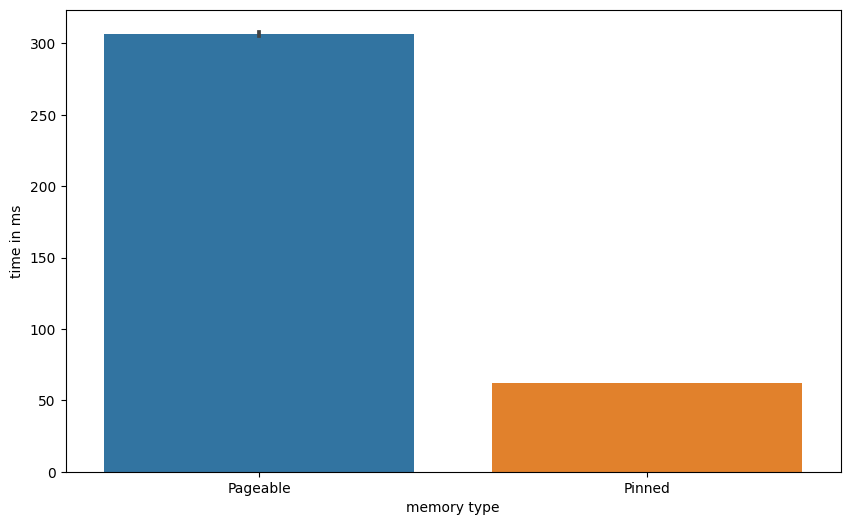
\includegraphics[width=0.98\linewidth]{read.png}
  \caption{Pagable vs Pinned memory}
  \label{fig:memory}
\end{figure}

\begin{figure}[H]
  \centering
  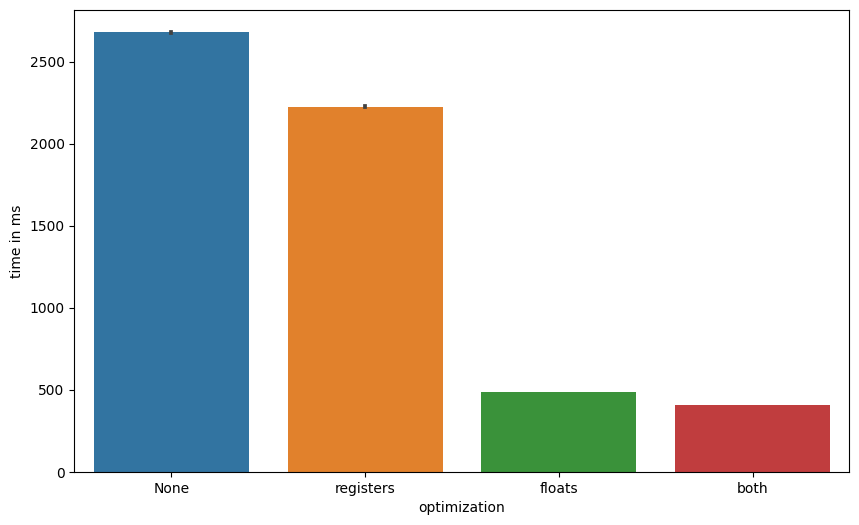
\includegraphics[width=0.98\linewidth]{run.png}
  \caption{GPU optimizations}
  \label{fig:optimizations}
\end{figure}

\begin{figure}[H]
  \centering
  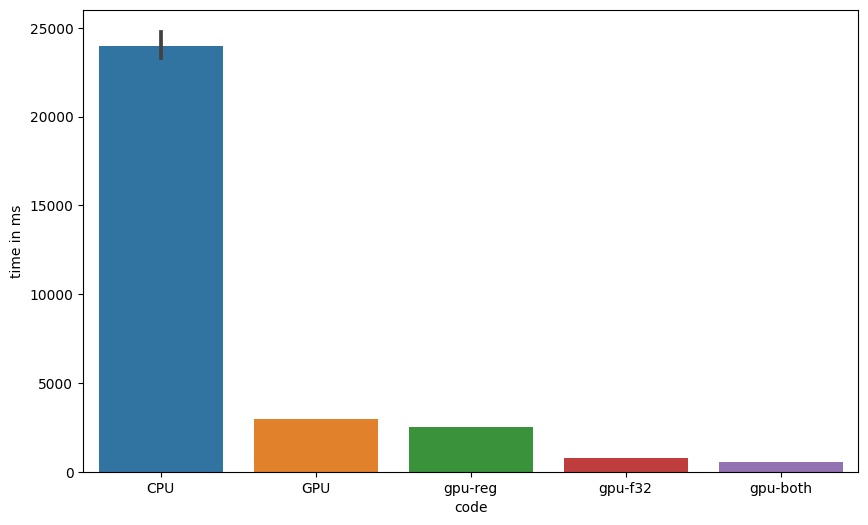
\includegraphics[width=0.98\linewidth]{cpu_vs_gpu.png}
  \caption{CPU vs GPU}
  \label{fig:cpu_vs_gpu}
\end{figure}

\hfill\\

\begin{table}[H]
    \begin{center}
    \begin{tabular}{ |l|c|c|} 
     \hline
      & E[ms] & E[seconds] \\ \hline
      cpu & 24750ms & 24.5s   \\ \hline
      gpu  & 2968ms & 2.9s  \\ \hline
      gpu-pinned & 2676ms & 2.6s  \\ \hline
      gpu-reg  & 2536ms & 2.5s  \\ \hline  
      gpu-f32  & 800ms & 0.8s  \\ \hline  
      gpu-all  & 512ms & 0.5s  \\ \hline  
     \hline
    \end{tabular}
     \label{table:}
      \caption{Table of figure \ref{fig:cpu_vs_gpu}}
    \end{center}
   
\end{table}

\section{Discussion}%
\label{sec:discussion}

In figure \ref{fig:cpu_vs_gpu} we are benchmarking the entire Mandelbrot generation (except
writing to file) this means that memory transfer from device to host is included. We can see
that a naive implementation is about 8.5 times faster than CPU, meanwhile my optimized
implementation is about 50x faster than CPU and 6x faster than the naive GPU.

The biggest performance boost was given by using f32 instead of f64, but using pinned memory
instead of Pageable memory made the memory transfer 5x faster. But memory transfer only
accounted for a small part of the full computation time. Using optimizations to make better
use of registers gave an additional performance boost of 20\%, both for f64
and f32.

In appendix I provide an example of the giant Mandelbrot image. Because of its size I cannot
provide an original image and will provide down-scaled variants of it. I also provide a link
here \href{..}{} to a Google drive file so you can download a version of the giant yourself
and inspect if you are interested.




\begin{thebibliography}{1}

  \bibitem{mandelbrot} Mandelbrot \url{https://en.wikipedia.org/wiki/Mandelbrot_set} \\2020-12-11 11:42:55.
  \bibitem{pinned memory} Pinned Memory
    \url{https://developer.nvidia.com/blog/how-optimize-data-transfers-cuda-cc/} \\2020-12-11 11:49:35
  \bibitem{cuda-version} Cuda toolkit
    \url{https://developer.nvidia.com/cuda-10.1-download-archive-base} \\2020-12-11 13:19:25
  \bibitem{cuda-registers} Cuda Registers
    \url{https://docs.nvidia.com/cuda/cuda-c-programming-guide/index.html#features-and-technical-specifications__technical-specifications-per-compute-capability}

\end{thebibliography}

\section{Appendix}%
\label{sec:appendinx}

\begin{figure}[H]
  \centering
  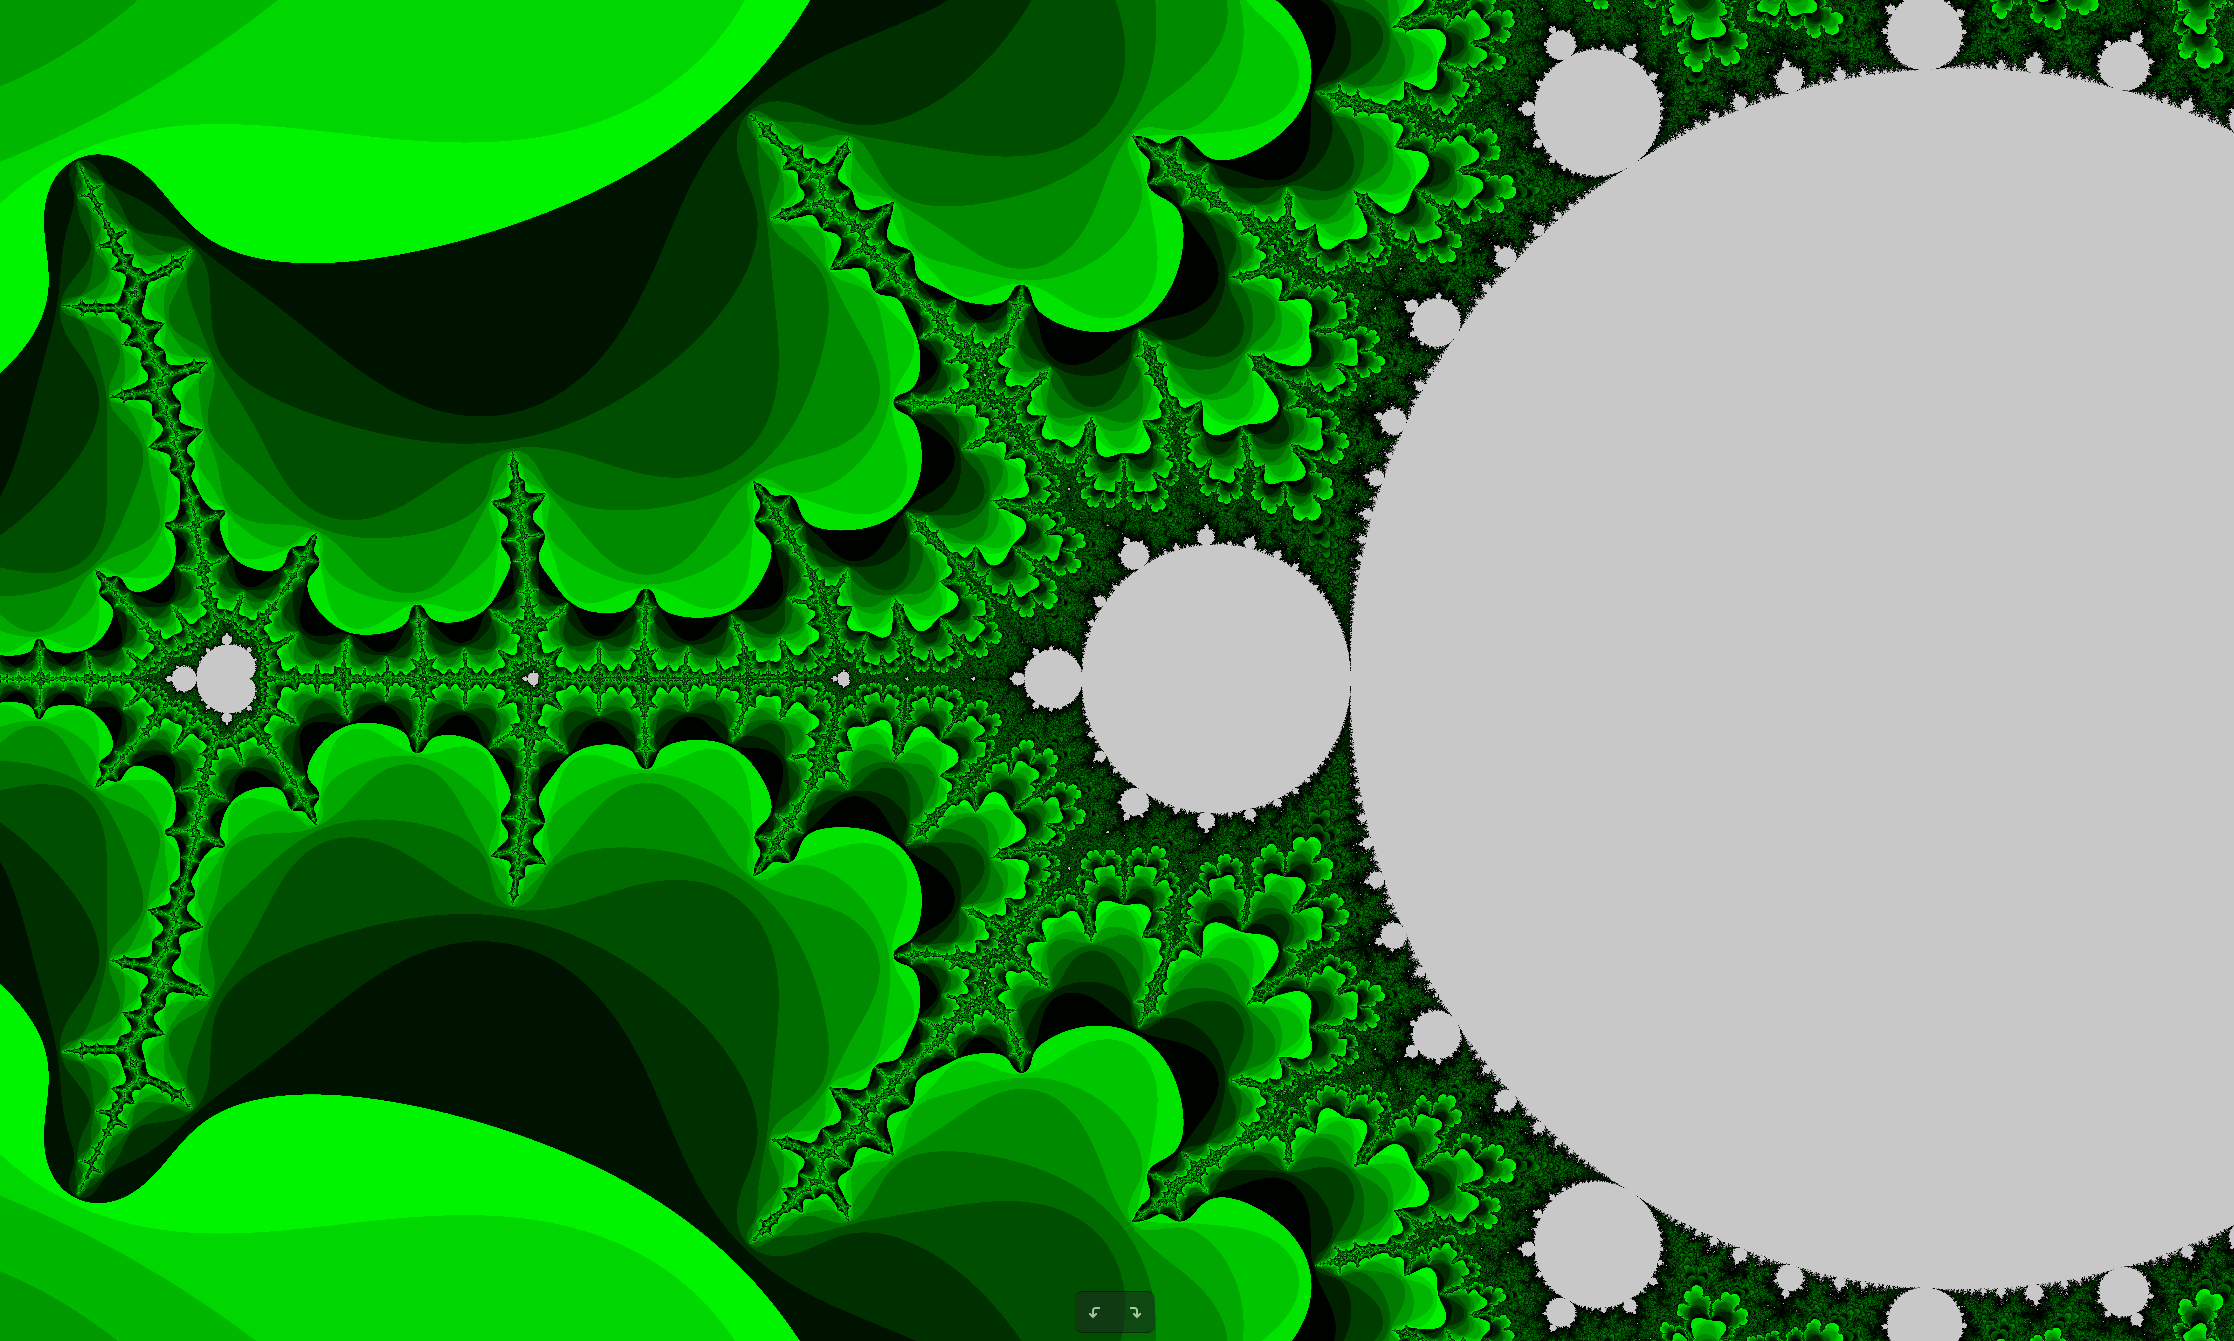
\includegraphics[width=0.48\linewidth]{original_mandelbrot.png}
  
\includegraphics[width=0.48\linewidth]{mandelbrot_zoom_1.png}
  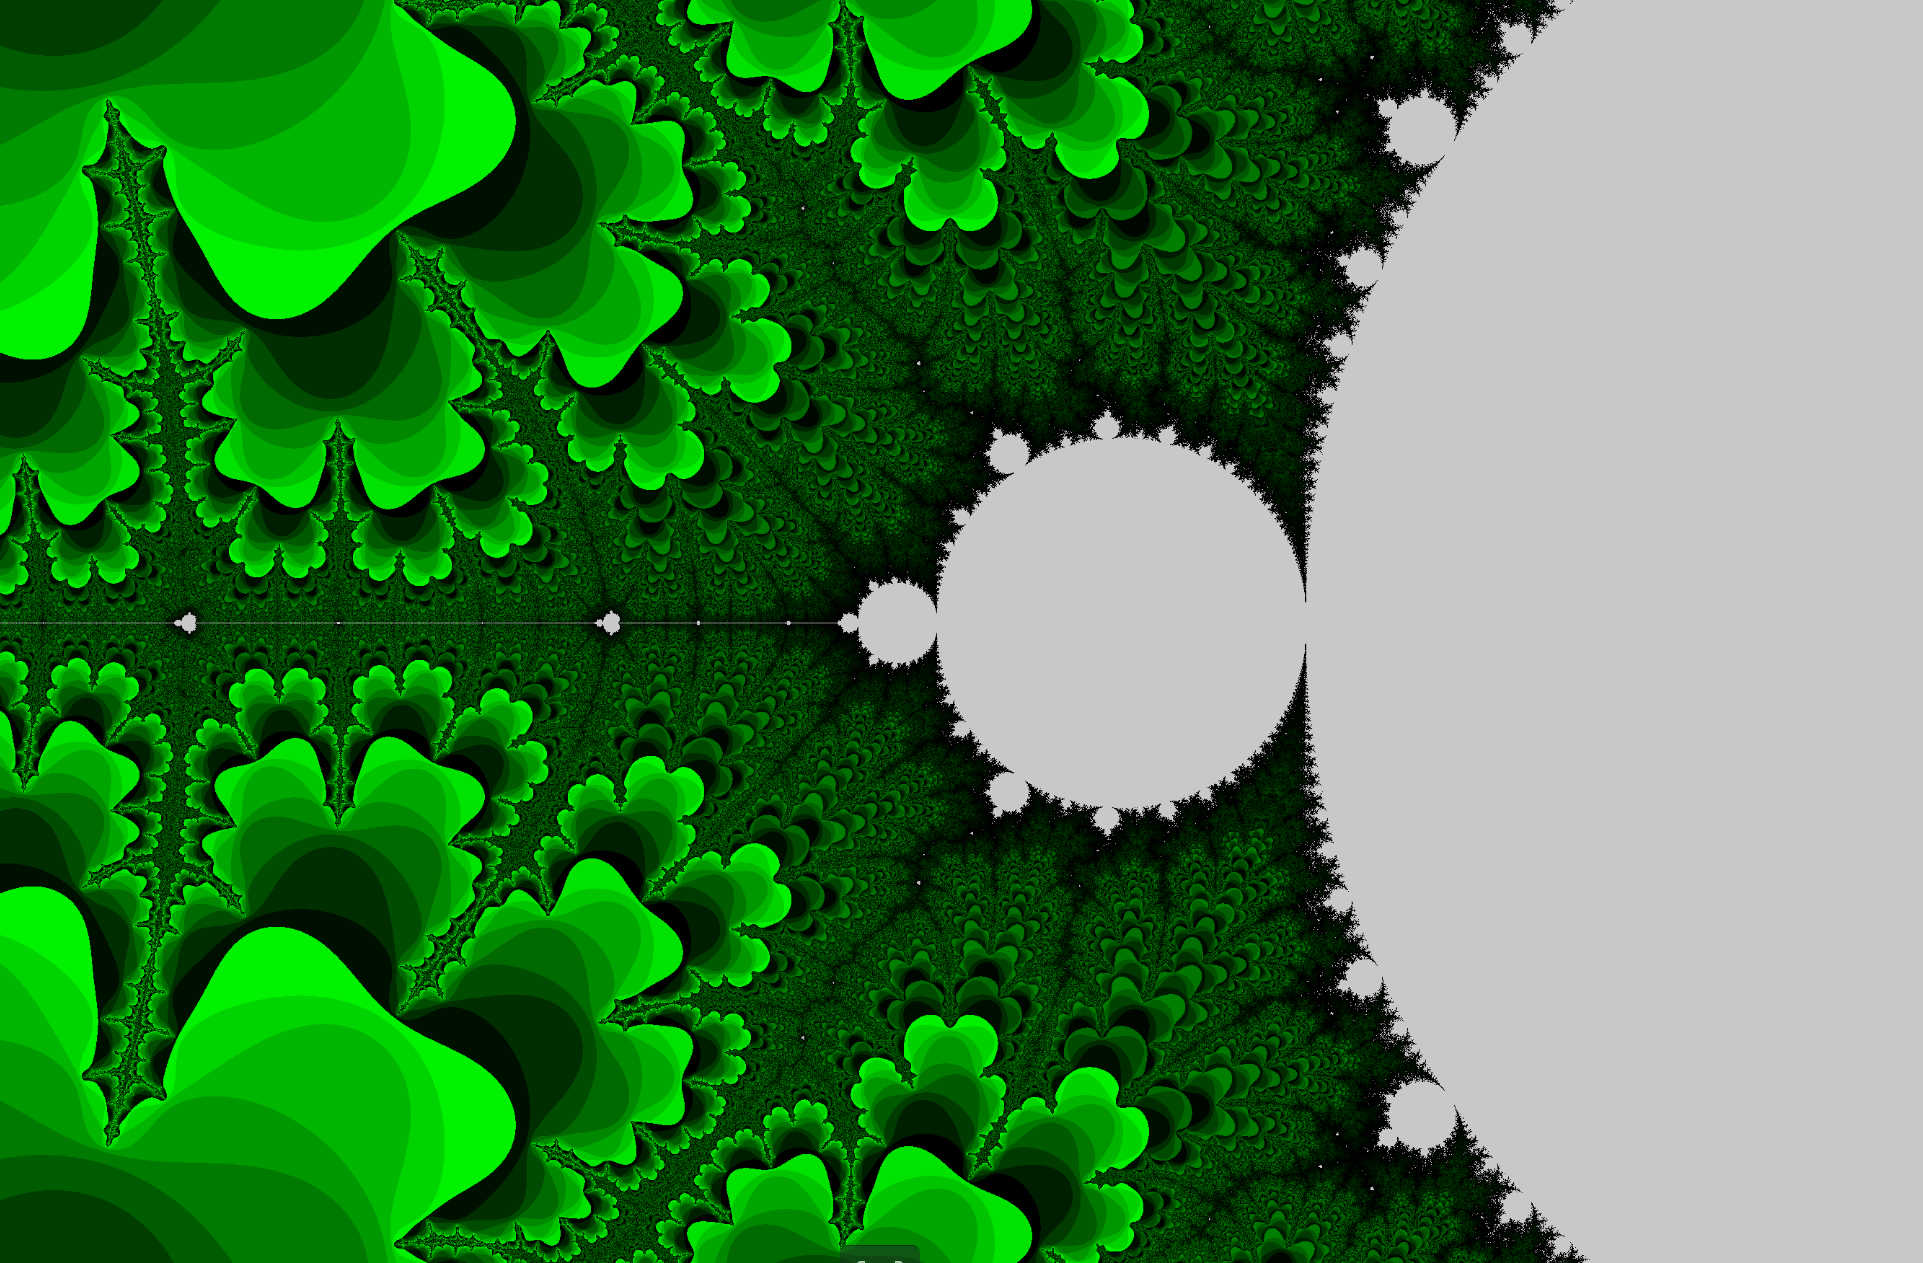
\includegraphics[width=0.48\linewidth]{mandelbrot_zoom_2.png}
  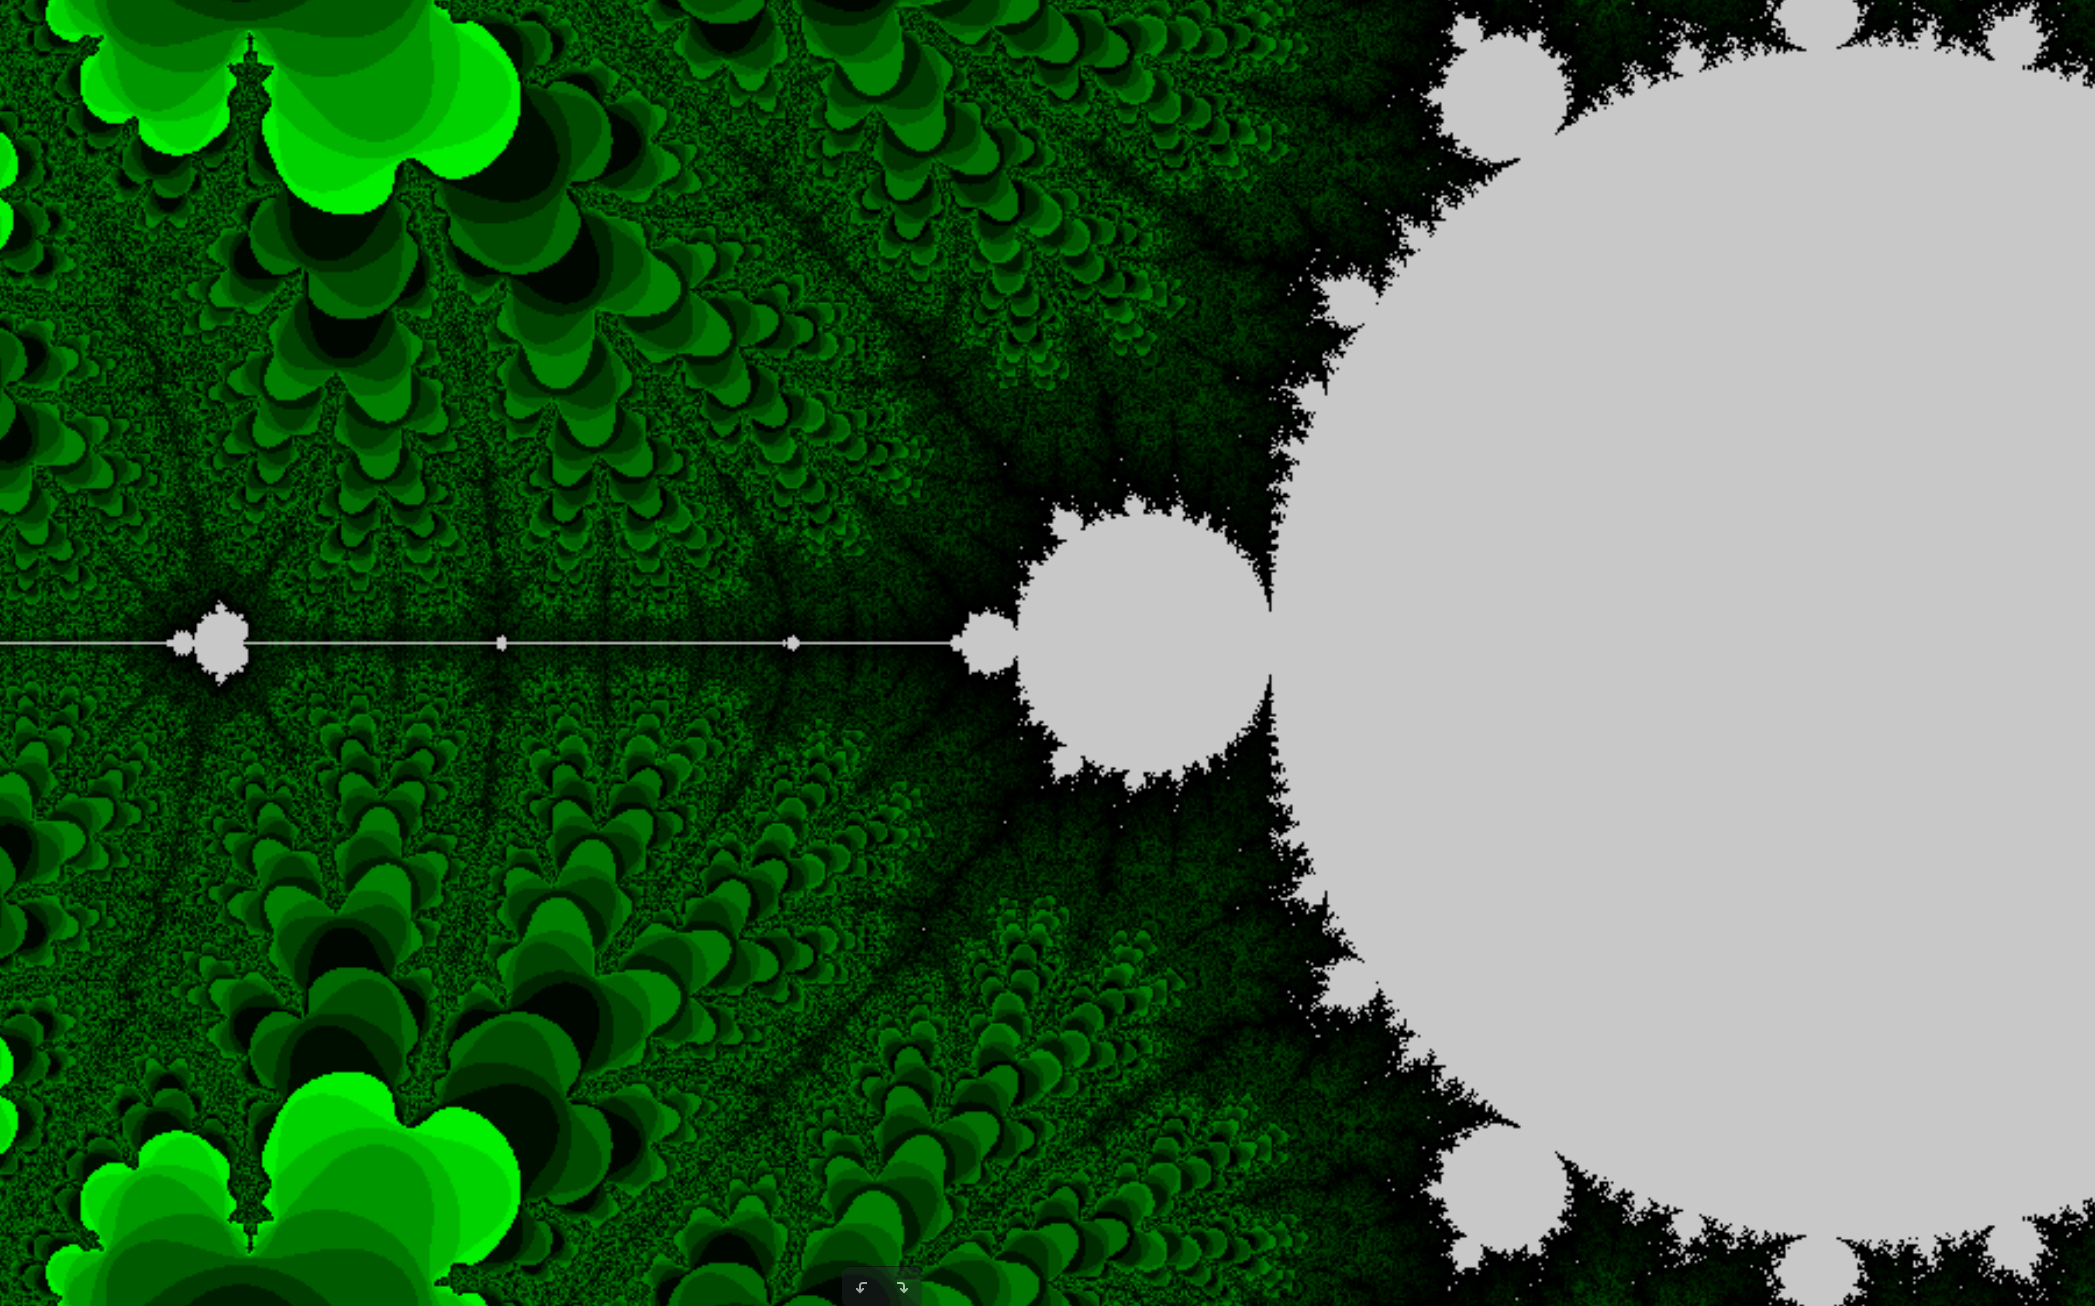
\includegraphics[width=0.48\linewidth]{mandelbrot_zoom_3.png}
\end{figure}

The top-left picture is the original image, the top-right is the image zoomed in on the first
bulb seen in the middle of the first. The bottom-left is zoomed in on the bulb seen in the
middle on the second and the bottom right is zoomed in on the bulb in the middle of the
bottom-left. On my 1920x1440 screen I started to be able to make out the pixels on the bottom
right one, but it is hard to see now on this small PDF.

Here is a zip file of the original image:\\
\href{https://drive.google.com/file/d/14C9NUHKD31HrKOdMnNovmTSdN5FFws-l/view?usp=sharing}{https://drive.google.com/file/d/14C9NUHKD31HrKOdMnNovmTSdN5FFws-l/view?usp=sharing}

Some programs might have trouble opening the original bmp file, since its is more than 1GB, so
I also included a jpg-file, that should be easy to open.

If you want to reproduce this exact file you just have to run the 

cuda\_mandel\_zoom.cu 


file.


Thank you for reading!


\end{document}




